Une étude a été réalisée sur la qualité de l'eau dans une région, en prélevant des échantillons dans deux types de milieux : des rivières et des lacs. Chaque échantillon a ensuite été analysé et classé comme de qualité \og satisfaisante \fg{} ou \og insatisfaisante \fg{} selon les normes en vigueur.

Voici les données recueillies à partir d'un total de 500 échantillons analysés :
\begin{itemize}
	\item 300 échantillons provenaient de rivières ;
	\item parmi les échantillons prélevés dans les lacs, 80 étaient classés de qualité \og insatisfaisante \fg{} ;
	\item au total, 280 échantillons étaient classés de qualité \og satisfaisante \fg.
\end{itemize}

\begin{enumerate}
	\item Recopier et compléter le tableau suivant :

	\begin{center}
		\begin{tblr}{hlines, vlines, colspec={l*{3}{X[c,25mm]}}}
			& Rivière & Lac & Total \\
			Qualité satisfaisante & & & \\
			Qualité insatisfaisante & & & \\
			Total & & & 500 \\
		\end{tblr}
	\end{center}

	\item On choisit un échantillon d'eau au hasard parmi les 500 échantillons analysés.

	On note les évènements suivants :
	\begin{itemize}[left=5mm,label={}]
		\item $S$ : \og l'échantillon choisi est classé de qualité satisfaisante \fg{} ;
		\item $R$ : \og l'échantillon choisi provient d'une rivière \fg.
	\end{itemize}

	\emph{Pour un évènement quelconque $E$ : on note $\overline{E}$ l'évènement contraire de $E$ et $P(E)$ la probabilité de $E$.}

	On donnera les résultats sous forme de fraction.

	\begin{enumerate}
		\item Quelle est la probabilité que l'échantillon provienne d'une rivière ?
		\item Décrire l'évènement $\overline{S}$ par une phrase puis justifier que $P\left(\overline{S}\right) = \dfrac{11}{25}$.
		\item Calculer $P\left(S \cap \overline{R}\right)$, puis interpréter ce résultat dans le contexte de l'énoncé.
	\end{enumerate}

	\item La situation est représentée par l'arbre pondéré ci-dessous :

	\begin{center}
		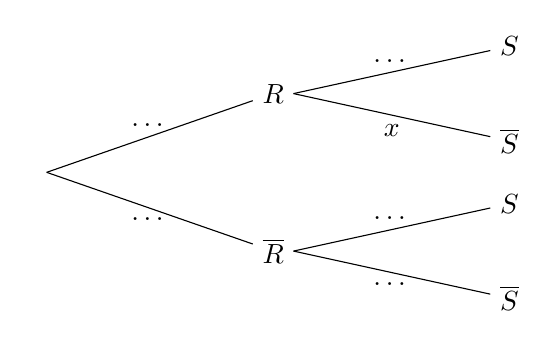
\begin{tikzpicture}[x=3cm, y=1cm]
			
			\node (root) at (0,0) {};
			\node (A) at (1,1) {$R$};
			\node (Abar) at (1,-1) {$\overline{R}$};
			\node (B1) at (2,1.6) {$S$};
			\node (B1b) at (2,0.4) {$\overline{S}$};
			\node (B2) at (2,-0.4) {$S$};
			\node (B2b) at (2,-1.6) {$\overline{S}$};
			
			\draw (root.east) -- (A) node[pos=0.5,above] {\ldots};
			\draw (root.east) -- (Abar) node[pos=0.5,below] {\ldots};
			
			\draw (A.east) -- (B1) node[pos=0.5,above] {\ldots};
			\draw (A.east) -- (B1b) node[pos=0.5,below] {$x$};
			\draw (Abar.east) -- (B2) node[pos=0.5,above] {\ldots};
			\draw (Abar.east) -- (B2b) node[pos=0.5,below] {\ldots};
		\end{tikzpicture}
	\end{center}

	\begin{enumerate}
		\item Traduire la probabilité $x$ en utilisant les évènements $\overline{S}$ et $R$.
		\item Vérifier que $x = \dfrac{7}{15}$.
		\item Recopier et compléter entièrement l'arbre.
	\end{enumerate}

	\item Les évènements \og l'échantillon provient d'une rivière \fg{} et \og l'échantillon est de qualité insatisfaisante \fg{} sont-ils indépendants ?
\end{enumerate}
